\chapter{Progettazione Concettuale}

\section{Premesse alla lettura dei diagrammi}

\subsection{Modelli Utilizzati}

Procediamo alla modellizzazione del mini-mondo, partendo dalla progettazione concettuale.

Questa fase di progettazione è stata svolta utilizzando, oltre che il modello \textbf{UML} nella forma di un \textbf{Class Diagram}, anche il modello \textbf{EER}, ovvero \textbf{Enhanced Entity Relationship}, per cogliere meglio aspetti del dominio che un modello \textbf{ER} classico non avrebbe potuto cogliere, come ad esempio \textbf{generalizzazioni e specializzazioni}.

\subsection{Precisazioni sui Diagrammi}

\subsubsection{EER Diagram}

Vista la densità del diagramma \textbf{EER}, si è deciso d'introdurre un \textbf{color coding} per facilitarne la lettura:

\begin{itemize}
  \item \textcolor{PRIMARY}{Entità}, e dunque Specializzazioni in \textcolor{PRIMARY}{arancione};
  \item \textcolor{CONTRAST}{Relazioni} in \textcolor{CONTRAST}{celeste};
  \item \textcolor{NEWGREEN}{Attributi} in \textcolor{NEWGREEN}{verde};
\end{itemize}

Inoltre, in caso di accavallamento di linee, si è deciso d'interrompere la linea in secondo piano in corrispondenza di un intersezione, così da evidenziare i diversi collegamenti.

\subsubsection{UML Class Diagram}

Per migliorare la leggibilità dei diagrammi, si è deciso di specificare le \textbf{molteplicità} degli attributi esclusivamente per sottolineare la possibilità di essere valorizzato a \textbf{NULL}. 

In tali casi si è utilizzata la molteplicità \textbf{[\(0..1\)]} esclusivamente per gli attributi di tipo \textbf{Bool}, mentre \textbf{[\(0..*\)]} per gli altri.

\bigskip

\begin{note}[Leggibilità dei Diagrammi]
  In caso di problemi di leggibilità dei diagrammi, sono disponibili le versioni originali nella pagina GitHub del progetto:
  \exlink{https://github.com/RiccardoElena/UninaDelivery/blob/develop/db/docs/sources/ER_Diagram.pdf}{ER Diagram} e \exlink{https://github.com/RiccardoElena/UninaDelivery/blob/develop/db/docs/sources/UML_Class_Diagram.pdf}{UML Class Diagram}.
\end{note}

\newpage
% TODO @zGenny export the ER diagram with the new changes and uncommend this part

\section{Enhanced Entity Relationship Diagram}
\begin{center}
  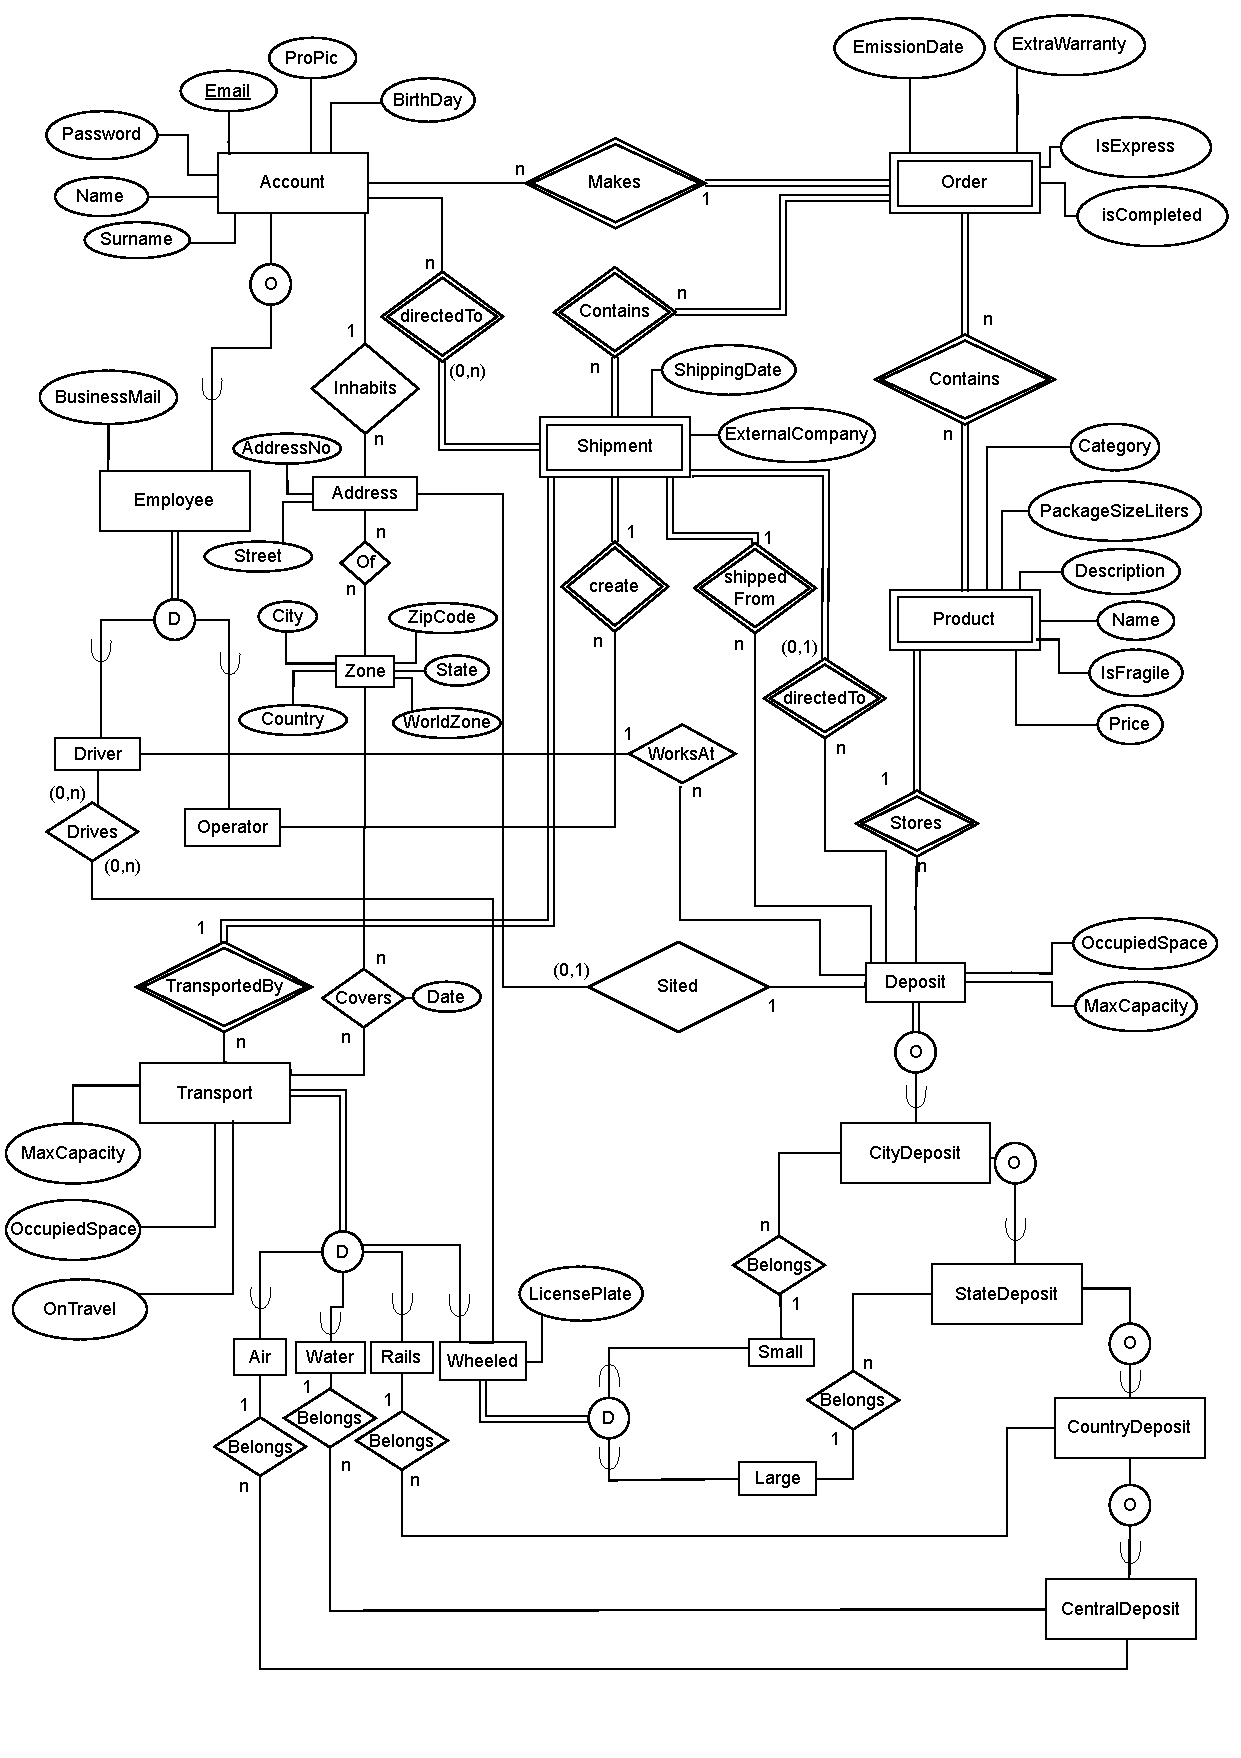
\includegraphics[width=0.9\textwidth]{ER_Diagram.pdf}
\end{center}

% TODO: need to re-export the UML diagram with the new changes. All the changes in the ER diagram are already done in the UML diagram
% If it's needed scale the size of the image with 0.x or 1.x near to \textwidth

\section{UML Class Diagram}
\begin{center}
  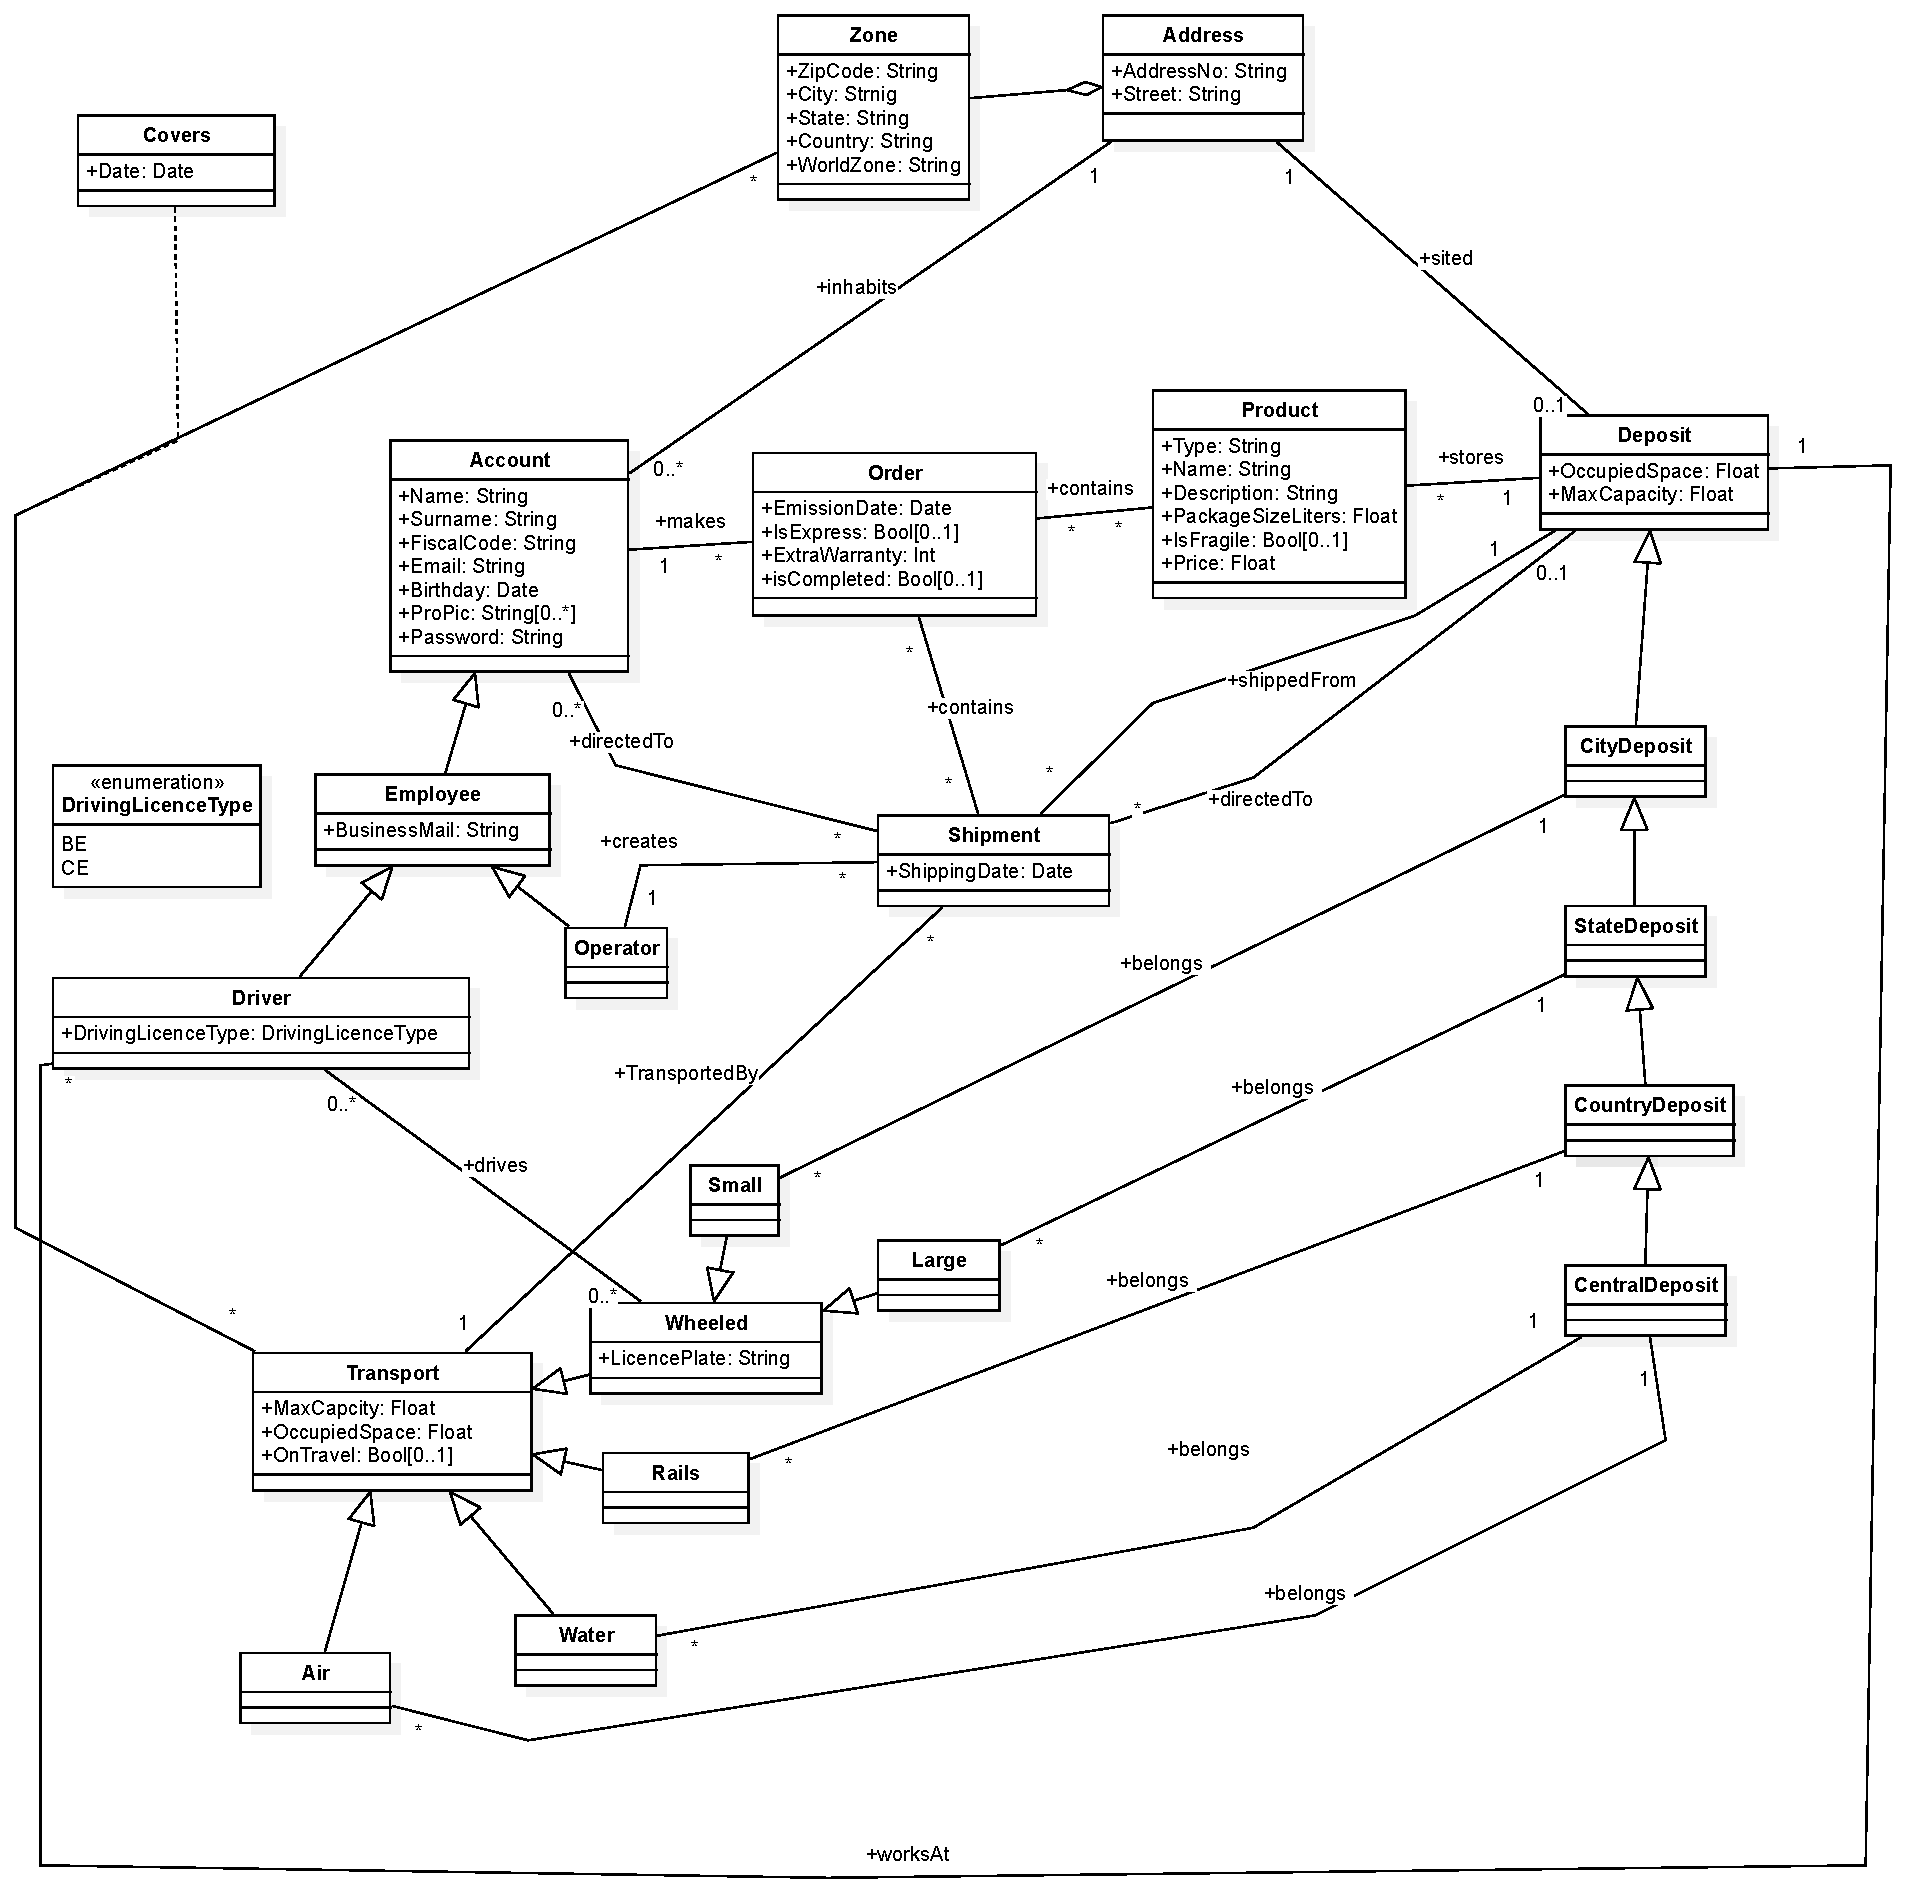
\includegraphics[width=\textwidth]{UML_Class_Diagram.pdf}
\end{center}

\newpage

\section{Ristrutturazione del Diagramma UML}

\subsection{Considerazioni sulla Ristrutturazione}

\subsubsection{Attributi Multipli e Multivalore}

Nello schema concettuale non sono presenti attributi \textbf{Multipli} o \textbf{Multivalore}, in quanto non sono stati ritenuti necessari per la rappresentazione del mini-mondo.

\subsubsection{Attributi Derivati}

Nello schema concettuale sono presenti due attributi \textbf{Derivati}:

\begin{itemize}
  \item L'attributo \textbf{Price} dell'entità \textbf{Shipment}, il quale però non ha necessità di essere conservato, non essendo un attributo di frequente richiesta per il sistema richiesto, e che quindi può essere eventualmente calcolato \textit{on-the-fly} in fase d'interrogazione del database basandosi sugli indirizzi di partenza e arrivo della spedizione e sulle eventuali modalità extra di consegna specificate in \textbf{Order}, come \textit{ExtraWarranty} e \textit{IsExpress}.
  \item L'attributo \textbf{IsCompleted} dell'entità \textbf{Order}, invece, si è scelto di conservarlo, in quanto è un attributo che può essere richiesto frequentemente dal sistema, e richiede un controllo relativamente complesso per essere valorizzato. Un ordine è considerato \textit{completato} se tutti i prodotti che contiene sono stati consegnati all'utente, dunque sarebbe necessario infatti controllare che tutti i prodotti dell'ordine siano stati spediti al destinatario, e che tali spedizioni siano andate a buon fine, coinvolgendo ben quattro entità: \textbf{Order}, \textbf{Product}, \textbf{Shipment} e \textbf{Account}. % * We should add a trigger that does this the first time
  \item L'attributo \textbf{OccupiedSpace} sia dell'entità \textbf{Deposit} che dell'entità \textbf{Transport}, infine, è stato anch'esso conservato, in quanto è un attributo che può essere richiesto frequentemente dal sistema, e richiede un interrogazione con risultato potenzialmente molto grande per essere valorizzata. % * this can be a cool trigger too.
\end{itemize}

\subsubsection{Generalizzazioni e Specializzazioni}

Le varie \textbf{Generalizzazioni} e \textbf{Specializzazioni} presenti nello schema concettuale sono state ristrutturate usando metodologie diverse, in base alla loro natura.

\begin{itemize}
  \item[\textbf{Employee:}] Essendo la specializzazione \textbf{Totale Disgiunta}, ed essendo le classi coinvolte in poche associazioni, si è scelto di accorpare la classe generale in quelle specializzate.
  \item[\textbf{Account:}] Essendo la specializzazione \textbf{Parziale Overlapping}, si è deciso di trasformarla in \textbf{Associazione}, limitando così il più possibile il numero di campi \textbf{NULL} e di \textbf{Vincoli d'Integrità}.
  \item[\textbf{Deposit:}] In questo caso trattandosi di una gerarchia di specializzazione si è scelto di accorpare a cascata le classi specializzate in quella generale, non avendo le classi specializzate attributi ed essendo tutte coinvolte in un'unica associazione concettualmente identica che verrà successivamente analizzata.
  \item[\textbf{Transport:}] Analogamente a quanto visto per \textbf{Deposit}, nonostante non si tratti di una gerarchia, si è scelto di accorpare le classi specializzate in quella generale. 
\end{itemize}

\subsubsection{Analisi delle Ridondanze}\label{Redundancy analysis}

Vediamo infine le ridondanze presenti nello schema concettuale, e come sono state rimosse.

Dalla ristrutturazione delle \textbf{Specializzazioni} di \textbf{Transport} sono emersi quattro attributi che servono essenzialmente lo stesso scopo ma per tipologie diverse di mezzi di trasporto: \textbf{Licence Plate}, \textbf{TrainNo}, \textbf{IMOCode} e \textbf{FlightNo}. Si è quindi deciso di accorpare questi attributi in un unico attributo \textbf{TransportID}, che può essere valorizzato con un identificativo univoco condiviso tra le tipologie di mezzi di trasporto, eliminando la possibilità di valori \textbf{NULL} o di valori uguali per tipi di mezzi diversi che imponevano aggiunta di vincoli o presenza di più attributi.

Inoltre la ristrutturazione delle \textbf{Specializzazioni} di \textbf{Deposit} ha fatto emergere quattro associazioni identiche a meno di vincoli che le riguardano, ovvero le associazioni \textbf{belongs}. È possibile dunque ridurle a un'unica associazione preservando i vincoli.

In ultima analisi, la classe \textbf{Shipment} è coinvolta in due associazioni semanticamente identiche, che si distinguono solo per molteplicità e seconda classe coinvolta, ovvero \textbf{Account} e \textbf{Deposit}. In particolare quella con \textbf{Account} è un'associazione circolare, essendo entrambe le classi associate anche con \textbf{Order}. Si è quindi deciso di eliminare l'associazione con \textbf{Account}, essendo il destinatario della spedizione già noto tramite \textbf{Order}.

\subsection{Identificazione delle Chiavi primarie}

Aldilà delle chiavi primarie già presenti nello schema concettuale esplicitate nel \textbf{diagramma ER} e dell'attributo \textbf{TransportID} introdotto \intlink{Redundancy analysis}{precedentemente}, si è deciso di aggiungere chiavi surrogate per le entità \textbf{Order}, \textbf{Shipment} e \textbf{Deposit}, poiché migrando le chiavi di altre entità si sarebbero ottenute chiavi composte troppo lunghe e complesse.

Per l'entità \textbf{Address} invece, è risultato più appropriato migrare la chiave primaria di \textbf{Zone} essendo una composizione e di conseguenza già concettualmente una \textit{parte} dell'entità \textbf{Address}. 

\newpage

\subsection{Class Diagram Ristrutturato}

% TODO: @zGenny review restructured diagram, if it's ok export it and uncommend this part. To adjust size add 0.x or 1.x near to \textwidth

% \begin{center}
  % ! USE THE NAME MENTIONED HERE FOR THE FILE
%   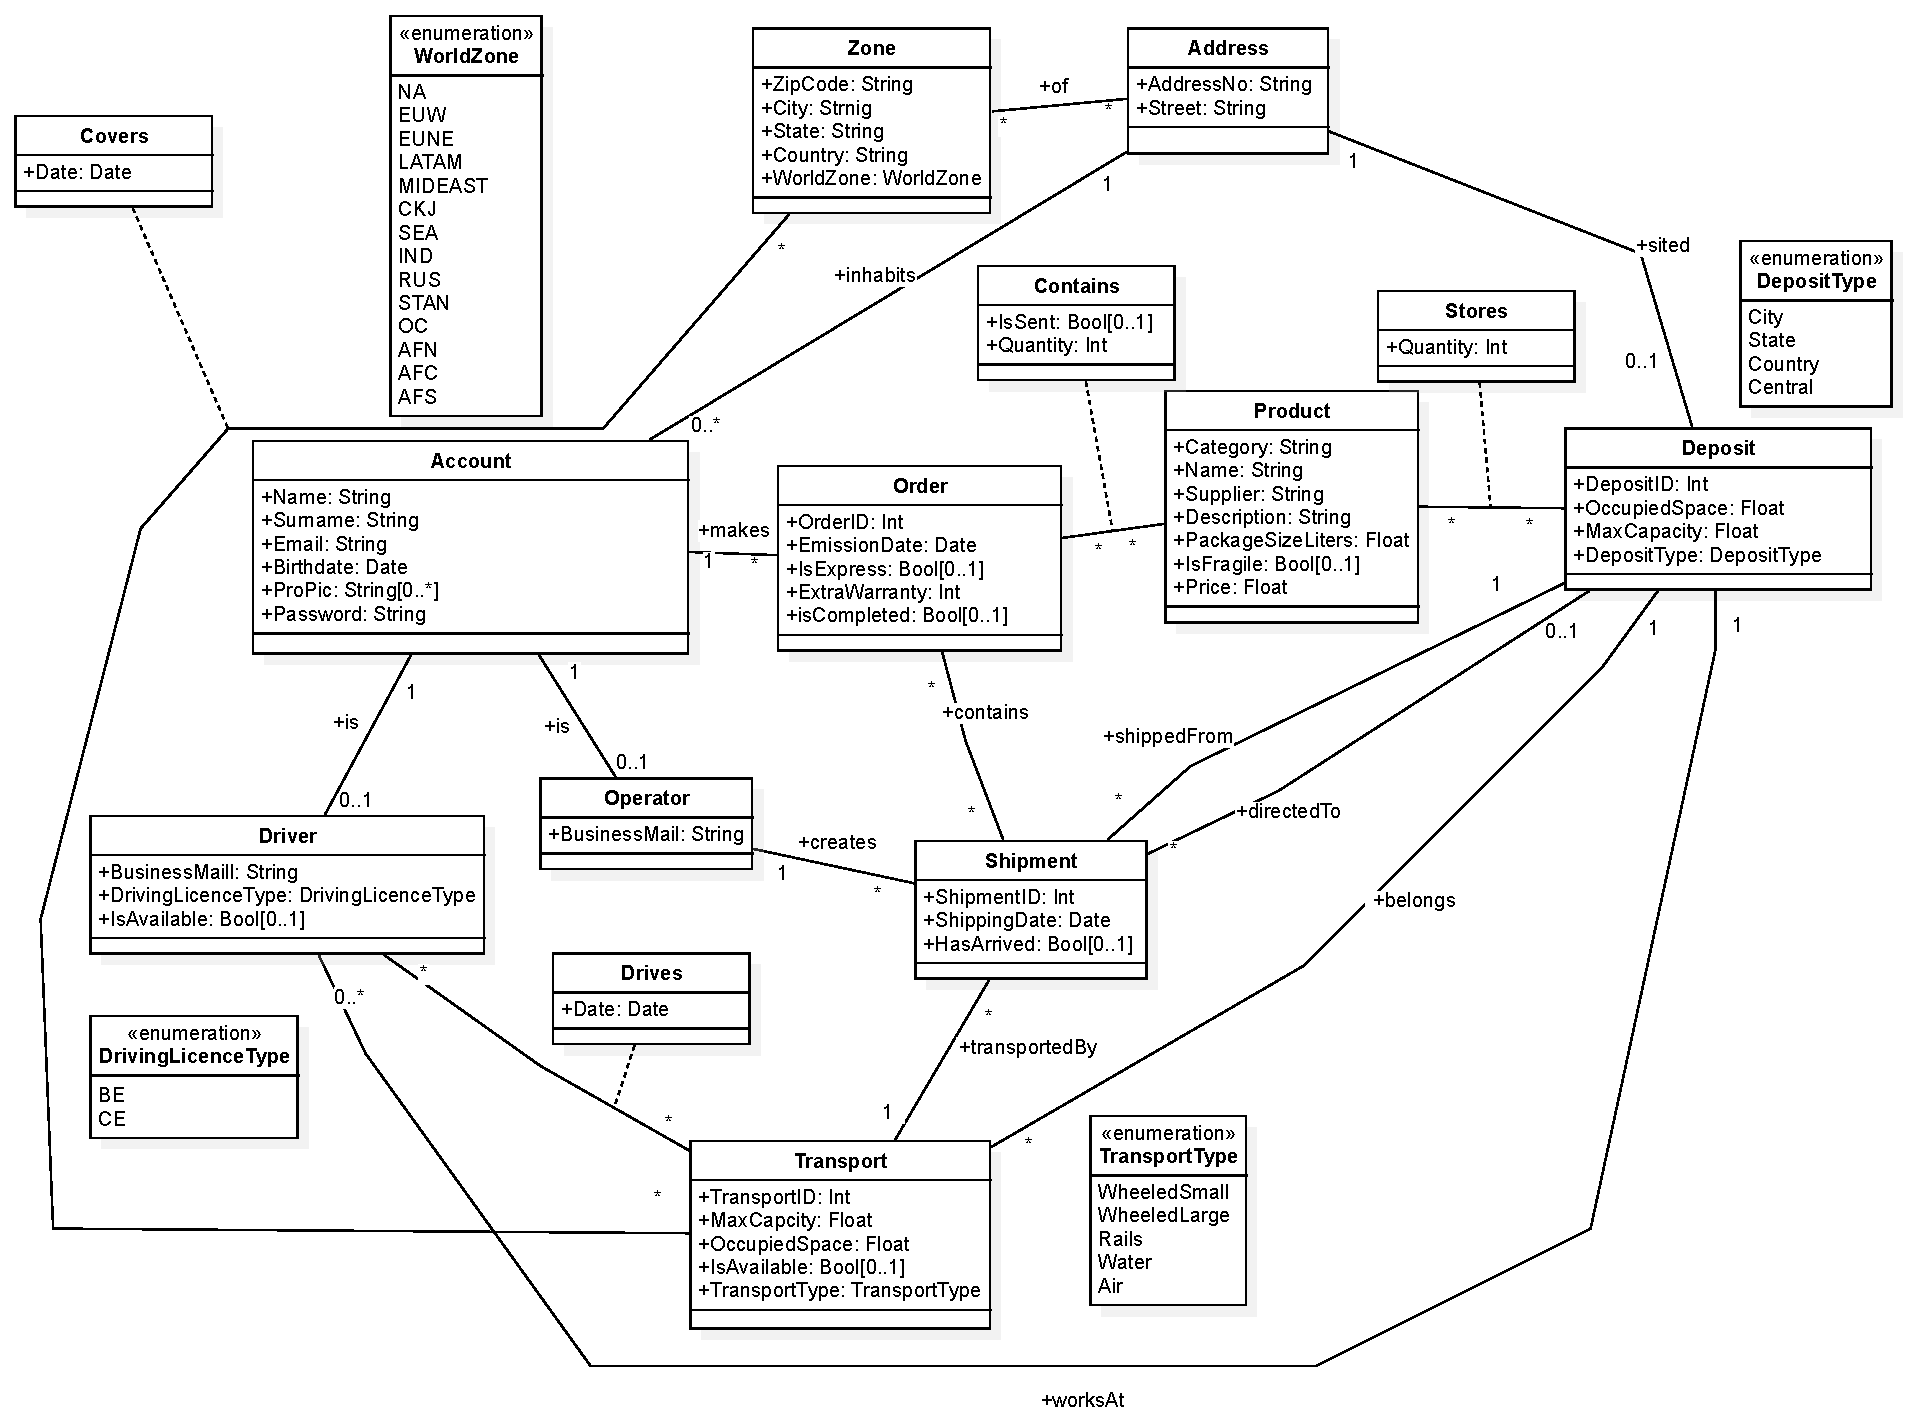
\includegraphics[width=\textwidth]{UML_Class_Diagram_Restructured.pdf} 
% \end{center}

\newpage

\section{Dizionari}

\subsection{Dizionario delle Classi}

\customTable{cYY}[Dizionario delle classi Prima Parte]{\textbfB{Classe} & \textbfB{Descrizione} & \textbfB{Attributi}}{
  \textbf{Account} & Generico utente che utilizza il sistema per effettuare ordini. & 
  {\footnotesize 
  \textbf{Name:} (\textit{string}): Nome dell'utente;
  
  \textbf{Surname} (\textit{string}): Cognome dell'utente;
  
  \textbf{Email} (\textit{string}): Chiave Primaria. Email dell'utente;

  \textbf{Birthdate} (\textit{date}): Data di nascita dell'utente;

  \textbf{ProPic} (\textit{string}): Eventuale immagine profilo dell'utente;

  \textbf{Password} (\textit{string}): Password dell'utente;  
  }\\


  \textbf{Operator} & Account di un impiegato che si occupa di creare le spedizioni. &
  {\footnotesize
  \textbf{BusinessMail} (\textit{string}): Chiave Primaria. Email aziendale dell'operatore;
  }\\


  \textbf{Driver} & Account di un autista che si occupa di effettuare le consegne. &
  {\footnotesize
  \textbf{BusinessMail} (\textit{string}): Chiave Primaria. Email aziendale dell'autista;

  \textbf{DrivingLincenceType} (\textit{DrivingLincenceType}): Tipologia di patente dell'autista;

  \textbf{IsAvailable} (\textit{bool}): Indica se l'autista è disponibile o meno;
  }\\


  \textbf{Order} & Ordine effettuato da un utente. Può contenere più prodotti e può essere spedito in più spedizioni. &
  {\footnotesize
  \textbf{OrderID} (\textit{integer}): Chiave Surrogata. Identificativo dell'ordine;

  \textbf{EmissionDate} (\textit{date}): Data di emissione dell'ordine;

  \textbf{IsExpress} (\textit{bool}): Indica se l'ordine è espresso o meno;

  \textbf{ExtraWarranty} (\textit{bool}): Indica se è stata acquistata una garanzia extra o meno;

  \textbf{IsCompleted} (\textit{bool}): Indica se l'ordine è stato completato o meno;
  }\\


  \textbf{Shipment} & Singola spedizione partita da un deposito. Può contenere più ordini e può raggiungere a più utenti o a un deposito. &
  {\footnotesize
  \textbf{ShipmentID} (\textit{integer}): Chiave Surrogata. Identificativo della spedizione; 

  \textbf{ShippingDate} (\textit{date}): Data della spedizione;
  }\\  
}

\newpage

\customTable{cYY}[Dizionario delle classi Seconda Parte]{\textbfB{Classe} & \textbfB{Descrizione} & \textbfB{Attributi}}{
  \textbf{Product} & Prodotto acquistabile da un utente. Può essere conservato in più depositi. &
  { \footnotesize
    \textbf{Type} (\textit{string}): Categoria del prodotto;

    \textbf{Name} (\textit{string}): Chiave Primaria. Nome del prodotto;

    \textbf{Supplier} (\textit{string}): Chiave Primaria. Fornitore del prodotto. Di default è \textit{UninaDelivery};
  
    \textbf{Description} (\textit{string}): Descrizione del prodotto;

    \textbf{PackageSizeLiters} (\textit{float}): Dimensione del prodotto in litri;

    \textbf{IsFagile} (\textit{bool}): Indica se il prodotto è fragile o meno;

    \textbf{Price} (\textit{float}): Prezzo del prodotto;
  }\\


  \textbf{Deposit} & Deposito per la conservazione di prodotti. Può contenere più prodotti e può essere raggiunto da più spedizioni. &
  {\footnotesize
  \textbf{DepositID} (\textit{integer}): Chiave Surrogata. Identificativo del deposito;

  \textbf{OccupiedSpace} (\textit{float}): Spazio del deposito attualmente occupato;

  \textbf{MaxCapacity} (\textit{float}): Spazio massimo del deposito;

  \textbf{DepositType} (\textit{DepositType}): Tipologia del deposito;
  }\\
  

  \textbf{Zone} & Zona del mondo raggiungibile da un mezzo di trasporto. Contiene più indirizzi. &
  {\footnotesize
  \textbf{ZipCode} (\textit{string}): Chiave Primaria. Codice di Avviamento Postale della zona;

  \textbf{City} (\textit{string}): Città in cui si trova la zona;

  \textbf{Country} (\textit{string}): Chiave Primaria. Paese in cui si trova la zona;
  
  \textbf{WorldZone} (\textit{string}): Zona del mondo in cui si trova la zona;
  }\\

  \textbf{Address} & Indirizzo di un utente o di un deposito. & 
  {\footnotesize

  \textbf{AddressNo} (\textit{string}): Chiave Primaria. Numero civico dell'indirizzo; 

  \textbf{Street} (\textit{string}): Via dell'indirizzo;
  }\\

  \textbf{Transport} & Mezzo di trasporto utilizzato per le spedizioni. & 
  {\footnotesize
  \textbf{TransportID} (\textit{integer}): Chiave Surrogata. Identificativo del mezzo di trasporto;

  \textbf{MaxCapacity} (\textit{float}): Capacità massima del mezzo di trasporto;

  \textbf{OccupiedSpace} (\textit{float}): Spazio attualmente occupato dal mezzo di trasporto;

  \textbf{IsAvailable} (\textit{bool}): Indica se il mezzo di trasporto è disponibile o meno. Il campo sarà valorizzato a \textit{true} solo se il mezzo non è già in viaggio;
  
  \textbf{TransportType} (\textit{TransportType}): Tipologia del mezzo di trasporto;
  }\\

}

\newpage
\subsection{Dizionario delle Associazioni}

\customTable{cYYY}[Dizionario delle associazioni Prima Parte]{\textbfB{Associazione} & \textbfB{Descrizione} & \textbfB{Attributi} & \textbfB{Classi Coinvolte}}{
  Val 1 & Val 2 & Val 3 & Val 4 \\
  Val 1.2 & Val 2.2 & Val 3.2 & Val 4.2 \\
}
  

\newpage
\subsection{Dizionario dei Vincoli}

\customTable{ccY}[Dizionario dei vincoli Prima Parte]{\textbfB{Vincolo} & \textbfB{Tipologia} & \textbfB{Descrizione}}{
  Val 1 & Val 2 & Val 3 \\
  Val 1.2 & Val 2.2 & Val 3.2 \\
}




% TODO: @RiccardoElena @zGenny write this section
  % it should contains:
  % [x] all the considerations about the UML diagram
  % [x] the changes made to the UML diagram
  % [ ] the new UML diagram
  % [ ] constrints dictonary (table (?)). Styled as the example in the slides